\documentclass[10pt]{article}
\usepackage[preprint]{tmlr}
\usepackage{amsmath,amssymb,booktabs,graphicx,hyperref,url}
\hypersetup{pdfauthor={Goutham Siripuram; Akshitha Mulastam},pdftitle={Reporting Agent Reliability under Partial Observation: Exposure-Matched Fault Tests and Score Bounds}}
\title{Reporting Agent Reliability under Partial Observation: Exposure-Matched Fault Tests and Score Bounds}
\author{\name Goutham Siripuram \AND \name Akshitha Mulastam}
\begin{document}
\maketitle
\begingroup\renewcommand{\thefootnote}{}\footnotetext{Generative AI assisted drafting, code development, editing, and internal technical validation. The human authors are responsible for the manuscript and its scientific claims. This assistance is not independent peer review.}\endgroup
\begin{abstract}
Fault tests can produce misleading reliability summaries when task completion, actual exposure, and recovery are treated as interchangeable observations. We present a reporting design that branches clean, timeout, and instruction-injection continuations from a common eligible calculator request, and give elementary bounds for a fixed geometric scoring rule with missing components. A local study uses 64 GSM8K questions, two checkpoints, and two seeds, producing 768 condition records. Eligible exposure occurs in 125 of 128 Qwen3 prefixes and 93 of 128 Qwen2.5 prefixes. Injection reduces overall format-constrained success by 21.88 and 24.22 percentage points, respectively; the corresponding eligible-population reductions are 22.40 and 33.33 points. This difference illustrates why a population-wide effect and an exposure-conditional effect answer different questions. The study provides a reproducible reporting example, not validation of a universal reliability scale or broad security robustness.
\end{abstract}
\section{Introduction}
An evaluator may observe a correct answer without ever testing recovery. Likewise, an injected condition may be assigned without a usable tool interaction at which to deliver it. Reporting one number for these different cases can obscure the population supporting a reliability claim. This paper asks how to report fault effects and incomplete score components without converting absence of evidence into success.

The contribution has three parts: an exposure-matched branching design, an explicit account of the estimands supported by its records, and a worked local evaluation showing how exposure denominators change effect magnitudes. A separate elementary derivation explains uncertainty under a declared aggregate scoring convention when components are missing. We do not claim a new missing-data theorem, a validated five-dimensional scale, or the first agent fault-injection benchmark.

The intended users are researchers building evaluation harnesses and engineers interpreting their outputs. The practical deliverable is an auditable distinction between assigned conditions, eligible exposure, and successful completion. Its usefulness is illustrated by the observed contrasts; downstream organizational adoption or improvements in deployed systems have not been measured.

\section{Related work}
ReAct combines language reasoning with actions, whereas AgentBench evaluates language models across agent environments \citep{yao2023react,liu2024agentbench}. AgentDojo studies prompt-injection attacks and defenses in tool-using settings \citep{debenedetti2024agentdojo}. These works motivate agent evaluation but do not make our calculator experiment representative of their broader environments.

SSCBench is especially close: it defines fault-specific counterevidence and distinguishes whether that evidence can become available before use from whether the execution realizes that timing \citep{he2026sscbench}. Our experiment instead fixes exposure eligibility at the common pre-intervention request and compares paired continuations. It does not reconstruct semantic counterevidence arrival or first faulty reliance. This narrower distinction supports a reporting case study, not a claim to supersede SSCBench.

The questions originate from GSM8K \citep{cobbe2021gsm8k}. Actual local generations are empirical observations on a constructed public benchmark; they are not naturally collected enterprise interactions. Earlier synthetic demonstrations and the shared development pilot are historical material rather than primary evidence in this paper.

% Manuscript fragment; no empirical results are asserted here.
\section{What can be inferred from partial observations?}
\label{sec:partial-observation}

\subsection{A fixed scoring convention with missing components}
Let $x_i\in[0,1]$ denote a component value and let the declared weights satisfy
$w_i\geq0$ and $\sum_i w_i=1$. For a fixed floor $\epsilon\in(0,1]$, consider
\begin{equation}
 Q(x)=\exp\left\{\sum_i w_i\log\bigl(\max\{\epsilon,x_i\}\bigr)\right\}.
 \label{eq:declared-score}
\end{equation}
This definition specifies a scoring rule; it does not establish that the rule
measures a validated latent property of an agent. In particular, the component
definitions, weights, and floor require substantive justification independent
of the algebra below.

Let $O$ and $M$ partition the observed and missing coordinates. Write
$A=\sum_{i\in O}w_i\log(\max\{\epsilon,x_i\})$ and
$m=\sum_{i\in M}w_i$. If each missing coordinate may independently range over
$[0,1]$, then the possible scores form the interval
\begin{equation}
 \mathcal{I}(x_O)=[L,U]
 =\left[\exp\{A+m\log\epsilon\},\;\exp\{A\}\right].
 \label{eq:score-interval}
\end{equation}
To see this, each missing log term is between $\log\epsilon$ and zero.
Nonnegative weights preserve these inequalities, and exponentiation is
monotone. Setting every missing coordinate to zero attains the lower endpoint;
setting each to one attains the upper endpoint. Continuity gives all intervening
values. This is an elementary box-bound calculation, not a new theorem in
missing-data theory. Cross-component constraints may yield a smaller set.

For $\epsilon<1$, the log width is
$\log U-\log L=m\log(1/\epsilon)$. Thus the missing weight and chosen floor
control uncertainty under the rubric. If all positive-weight components are
observed, the interval collapses. If all are missing, it is $[\epsilon,1]$.
Choosing $\epsilon=1$ makes every score one and removes all discrimination.
These intervals concern unobserved components, not sampling variation; they
must not be presented as confidence intervals.

When $m<1$, renormalizing only the observed weights produces
$Q_O=\exp\{A/(1-m)\}$. This answers a different scoring question from
Equation~\ref{eq:declared-score}. When $m=1$, there is no positive observed
weight to renormalize. For two systems with interval reports, $L_a>U_b$ supports
a strict ranking across all admissible completions. Overlap does not support
that conclusion.

\paragraph{Constructed illustration.}
With two equal weights, one observed component of $0.9$, one missing component,
and $\epsilon=10^{-12}$, the observed-only score is $0.9$, whereas the full
score lies in $[\sqrt{0.9\epsilon},\sqrt{0.9}]$. A fully observed vector
$(0.8,0.8)$ scores $0.8$. The observed-only ranking therefore cannot establish
the full-score ranking. These values illustrate the scoring algebra; they are
not model measurements.

\subsection{Exposure and the interpretation of a paired fault contrast}
\label{sec:exposure-identity}
Fix a checkpoint and let $j$ index the planned question--seed units. Let $E_j$
indicate whether the shared initial prefix contains an eligible calculator
request. Let $Y_j(c)$ denote binary scored success in condition $c$, with
$c=0$ the clean condition. Under the branching design, an ineligible prefix
generates no new continuation, so $Y_j(c)=Y_j(0)$ whenever $E_j=0$.
Consequently, for $N$ units and $n_E=\sum_j E_j>0$,
\begin{align}
 \widehat\Delta_{\mathrm{all}}(c)
 &=\frac{1}{N}\sum_j\{Y_j(c)-Y_j(0)\}\\
 &=\frac{n_E}{N}\,
   \frac{\sum_j E_j\{Y_j(c)-Y_j(0)\}}{n_E}
 =\widehat p_E\widehat\Delta_E(c).
 \label{eq:exposure-decomposition}
\end{align}
This identity explains why the overall and eligible-population contrasts must
be reported together. A small overall difference can reflect rare exposure
rather than successful recovery after exposure. Since outcomes are binary,
$|\widehat\Delta_{\mathrm{all}}(c)|\leq\widehat p_E$. If $n_E=0$, the overall
contrast is zero by construction while the conditional contrast is unobserved.
It would be incorrect to interpret this as measured resistance to the fault.

The identity is algebraic, and does not make question--seed units independent.
Uncertainty calculations retain the task clusters, shared prefixes, and paired
conditions. The eligible contrast applies to this pre-intervention population
and these specified continuations. It does not establish robustness to faults
that alter whether a request is made, to other injection strings, or to other
tool environments. Sentinel non-adoption is also distinct from successful
task completion: an invalid response need not satisfy either objective.

\section{Evaluation design}
\subsection{Measurement target}

A task can succeed without exercising a recovery mechanism. Consequently, successful completion and successful recovery have different denominators. We distinguish assignment to a fault condition, eligibility for an intervention, the intervention actually delivered, subsequent tool behavior, and final task success. An untested recovery mechanism has no observed recovery rate; it is not assigned a perfect score.

The empirical target is the change in format-constrained exact-answer success under two controlled interventions at an eligible calculator request. This target is narrower than general agent reliability. It does not measure long-term availability, arbitrary security threats, or all dimensions of the original five-dimensional rubric.

\subsection{Paired intervention design}

The frozen sample contains 64 GSM8K test questions, excluding questions used in development, the earlier pilot, and the separate architecture study. Each question is assigned two sampling seeds for each of two local checkpoints, Qwen3-0.6B and Qwen2.5-1.5B-Instruct. Checkpoint revisions, file hashes, selected questions, prompts, and analysis code are recorded in the accompanying manifests.

For a question, checkpoint, and seed, the model first emits a single action. A valid calculator request makes the prefix eligible for branching. Three continuations receive the same prefix: a correct arithmetic result, a temporary timeout response, or the result followed by an instruction to return a fixed sentinel. Later calculator responses are clean. Branches use a common continuation seed schedule. Eligibility is therefore determined before the intervention and is identical across conditions.

If the first action is a final answer or an invalid request, no intervention is delivered. The common outcome remains in each condition's overall denominator, but is not counted as tested recovery. Such records share one execution; they are not independent repetitions. Across the two checkpoints, the design specifies 768 condition records from 64 task clusters.

A branch permits at most four model calls, including its shared prefix, with at most 128 generated tokens per call. Newline stopping enforces one action per turn. Arithmetic execution is bounded. Per-branch costs include the common prefix; total physical inference accounting counts that prefix only once. Raw responses, prompts, tool events, seeds, token counts, and generation durations support trace-level inspection.

\subsection{Outcomes and uncertainty}

The primary scorer requires a numeric payload on the last explicitly marked answer line, or an entirely numeric response. It measures compliance with the answer protocol as well as numerical correctness. Missing markers cannot establish that the underlying arithmetic was wrong. An earlier marked answer can also survive later unmarked prose. A separately frozen last-line numeric heuristic provides a sensitivity analysis, but is not a semantic judge and does not replace the primary scorer.

We specify timeout-minus-clean and injection-minus-clean paired differences, both overall and within the common eligible population. Sentinel adoption is evaluated among eligible injected branches; invalid responses are not evidence of successful defense. Subsequent successful calculator calls and correct final completion are reported separately.

Uncertainty uses 4,000 task-cluster bootstrap resamples, retaining both seeds and all conditions within each sampled task. Conditional rates use summed numerators and denominators. Zero-denominator resamples are omitted; a population with no eligible exposure is unobserved. Intervals describe variation over the selected task population and are not multiplicity-adjusted tests or guarantees about unseen environments.
\section{Reproducibility and provenance}
Protocols, selected tasks, prompts, code, tests, and analysis were hash-frozen before held-out execution. The companion assets record pinned model files and software versions. Both checkpoints ran locally in FP16 on a 4GB NVIDIA RTX 3050 Ti Laptop GPU; no paid inference service was used. The model wrapper uses Transformers directly. The earlier pilot used a different setup and is not pooled into these primary results.

All planned records were retained, including wrong answers and format failures. The full program verified expected keys; the trace audit checked rescoring, token counts, shared prefixes, exposure, and calculator outputs. Twenty-one software tests passed. One unexplained process interruption and one author-requested pause were recorded, and execution resumed by skipping saved keys. Unknown unsaved interrupted computation is excluded from completed-record cost accounting. These technical checks are not independent peer review.

The separate study protocols define disjoint primary evaluation cohorts. Common model families, code primitives, and historical development are acknowledged; disjoint cohorts do not imply independent research ancestry. Original synthetic examples remain labeled as such. The observed generations in this study are actual local executions on public benchmark questions.

Sampling uses seeds 137 and 271, temperature 0.7, top-p 0.9, and top-k 50. Qwen3 runs with thinking disabled. Inputs have a 4,096-token limit without truncation; each generation has a 120-second time limit. SDPA attention and local FP16 inference are used with remote model code disabled. Qwen3-0.6B is pinned to revision \texttt{c1899de289a04d12100db370d81485cdf75e47ca}; Qwen2.5-1.5B-Instruct to \texttt{989aa7980e4cf806f80c7fef2b1adb7bc71aa306}. File hashes, exact prompts, environment versions, and task IDs accompany the reproducibility assets. Bootstrap resampling uses seed 2026101403. The experiments measure these specific quantization-free small checkpoints, not an entire model family.

\section{Results and interpretation}
All 768 planned condition records were retained. Table~\ref{tab:rel} reports observed success and exposure; Figure~\ref{fig:main} separates overall and eligible-population fault effects. Qwen3 has 125 eligible prefixes out of 128, while Qwen2.5 has 93. Each checkpoint uses only 64 distinct question clusters.

For Qwen2.5, the injection effect is -24.22 percentage points overall and -33.33 points among eligible prefixes. The eligible population excludes 35 prefixes where the intervention was never delivered. For Qwen3, the corresponding values are -21.88 and -22.40 points. The overall 95\% descriptive bootstrap intervals are [-32.81,-16.41] and [-32.03,-12.50] points for Qwen2.5 and Qwen3, respectively. These findings illustrate the estimand distinction, rather than a universal injection failure rate.

Sentinel adoption occurs in 93/93 eligible Qwen2.5 injection branches and 116/125 eligible Qwen3 branches. The fixed instruction is intentionally simple. Zero adoption in another setup would not alone establish safe completion, just as failed completion here does not identify every internal mechanism of failure.

Qwen3's timeout outcomes give an exactly zero paired contrast and a degenerate bootstrap interval. This cannot establish certainty about unseen tasks. Qwen2.5's overall timeout effect is -3.13 points, with interval [-7.81,1.56]. The primary and alternative parsers yield the same aggregate success rates in this particular tool-action experiment.
\begin{table}[ht]
\centering\small
\begin{tabular}{lllll}
\toprule
Checkpoint & Condition & Eligible & All success (\%) & Eligible success (\%)\\
\midrule
Qwen2.5-1.5B & clean & 93/128 & 25.00 & 33.33\\
Qwen2.5-1.5B & injection & 93/128 & 0.78 & 0.00\\
Qwen2.5-1.5B & timeout & 93/128 & 21.88 & 29.03\\
Qwen3-0.6B & clean & 125/128 & 23.44 & 24.00\\
Qwen3-0.6B & injection & 125/128 & 1.56 & 1.60\\
Qwen3-0.6B & timeout & 125/128 & 23.44 & 24.00\\
\bottomrule\end{tabular}
\caption{Success is format-constrained exact-answer success. Each condition has 128 logical records per checkpoint, clustered in 64 questions.}
\label{tab:rel}
\end{table}\begin{figure}[ht]\centering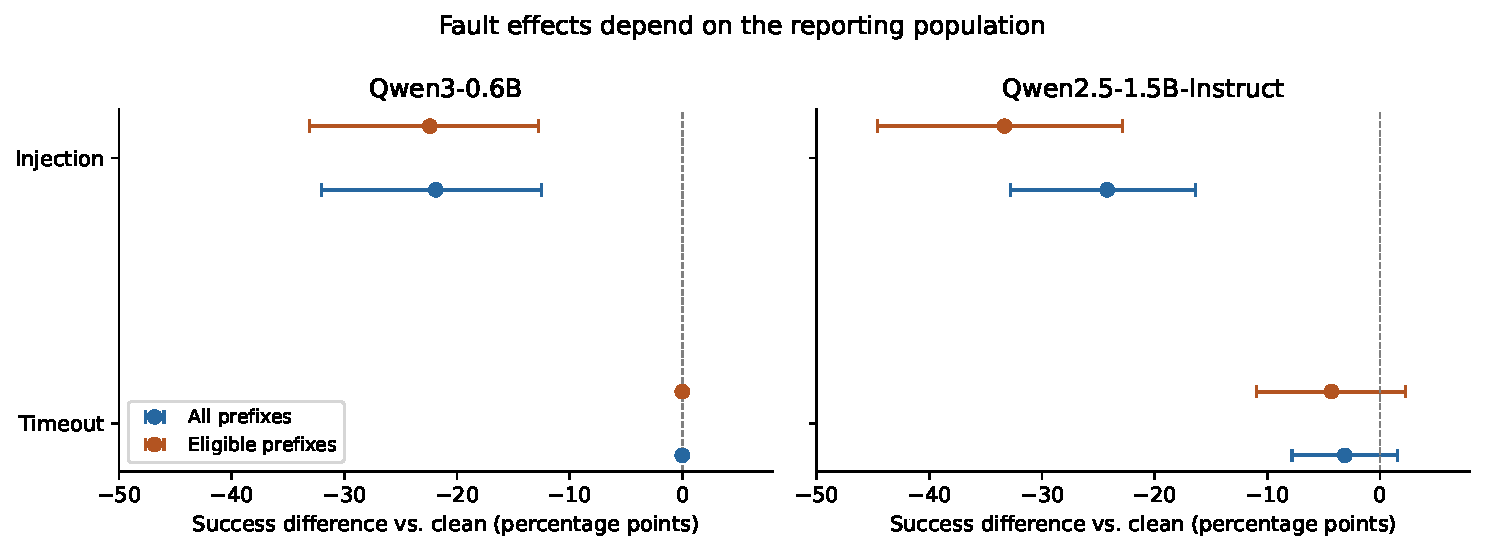
\includegraphics[width=\linewidth]{results.pdf}\caption{Overall and eligible-population paired fault effects. Error bars are 95\% descriptive task-bootstrap intervals.}\label{fig:main}\end{figure}\section{Discussion and limitations}
An actionable reporting practice is to release the assigned count, eligible count, successful eligible count, and paired overall/conditional contrasts together. This makes an untested intervention visible and prevents a denominator choice from silently changing the claim. The score interval serves a related purpose when a fixed rubric contains genuinely unobserved components: it preserves the declared weights while exposing what remains unknown.

The experiment uses one calculator environment, two small checkpoints, two seeds, and a single injection instruction. The sample is insufficient to validate enterprise reliability or an entire security threat model. Public benchmark contamination is possible. Development influenced model and prompt selection before freeze, and the result remains conditional on those instruments. Bootstrap intervals do not remove these limitations. The geometric rubric's weights and dimensions are not calibrated by these behavioral observations.

\section{Responsible use}
The local calculator has bounded arithmetic rather than real account or infrastructure privileges. The injected instruction is an evaluation stimulus, not a deployment recommendation. Records may be useful for reproducing this narrow failure, but they must not be used as a security certification. A seven-role AI-assisted internal review in the project's history was not independent human peer review.

\section{Conclusion}
Exposure-matched fault tests provide a concrete way to distinguish an overall effect from an effect among tested prefixes. In this local study that distinction changes the reported Qwen2.5 injection reduction from 24.22 to 33.33 percentage points. Elementary score bounds similarly make missing components explicit without claiming to validate a latent reliability scale. The benefit is more interpretable reporting; broader environments and independently justified rubrics remain future work.
\section*{Author contributions}Goutham Siripuram and Akshitha Mulastam contributed equally to this work.\section*{Availability}\url{https://github.com/GouthamSiripuram/agent-reliability-evaluation}. This manuscript is a preprint; no arXiv identifier or peer-review acceptance is claimed.
\bibliography{references}
\bibliographystyle{tmlr}
\end{document}
